\documentclass{article}

% Language setting
% Replace `english' with e.g. `spanish' to change the document language
\usepackage[spanish]{babel}

% Set page size and margins
% Replace `letterpaper' with `a4paper' for UK/EU standard size
\usepackage[a4paper,top=2cm,bottom=2cm,left=3cm,right=3cm,marginparwidth=1.75cm]{geometry}
\usepackage{pdfpages}
% Useful packages
\usepackage{amsmath}
\usepackage{graphicx}
\usepackage[colorlinks=true, allcolors=blue]{hyperref}
\usepackage{titling}
\usepackage{csquotes}
\usepackage[shortcuts]{extdash}
\usepackage[style=ieee,backend=biber]{biblatex}
\usepackage{imakeidx}
\usepackage{tikz}
\usepackage{tikz-uml}
\usepackage{caption}
\usepackage{listings}
\usepackage{xcolor}
\usetikzlibrary{babel}
\usetikzlibrary{positioning}


\makeatletter
\pgfkeys{/pgf/.cd,
  parallelepiped offset x/.initial=2mm,
  parallelepiped offset y/.initial=2mm
}
\pgfdeclareshape{parallelepiped}
{
  \inheritsavedanchors[from=rectangle] % this is nearly a rectangle
  \inheritanchorborder[from=rectangle]
  \inheritanchor[from=rectangle]{north}
  \inheritanchor[from=rectangle]{north west}
  \inheritanchor[from=rectangle]{north east}
  \inheritanchor[from=rectangle]{center}
  \inheritanchor[from=rectangle]{west}
  \inheritanchor[from=rectangle]{east}
  \inheritanchor[from=rectangle]{mid}
  \inheritanchor[from=rectangle]{mid west}
  \inheritanchor[from=rectangle]{mid east}
  \inheritanchor[from=rectangle]{base}
  \inheritanchor[from=rectangle]{base west}
  \inheritanchor[from=rectangle]{base east}
  \inheritanchor[from=rectangle]{south}
  \inheritanchor[from=rectangle]{south west}
  \inheritanchor[from=rectangle]{south east}
  \backgroundpath{
    % store lower right in xa/ya and upper right in xb/yb
    \southwest \pgf@xa=\pgf@x \pgf@ya=\pgf@y
    \northeast \pgf@xb=\pgf@x \pgf@yb=\pgf@y
    \pgfmathsetlength\pgfutil@tempdima{\pgfkeysvalueof{/pgf/parallelepiped offset x}}
    \pgfmathsetlength\pgfutil@tempdimb{\pgfkeysvalueof{/pgf/parallelepiped offset y}}
    \def\ppd@offset{\pgfpoint{\pgfutil@tempdima}{\pgfutil@tempdimb}}
    \pgfpathmoveto{\pgfqpoint{\pgf@xa}{\pgf@ya}}
    \pgfpathlineto{\pgfqpoint{\pgf@xb}{\pgf@ya}}
    \pgfpathlineto{\pgfqpoint{\pgf@xb}{\pgf@yb}}
    \pgfpathlineto{\pgfqpoint{\pgf@xa}{\pgf@yb}}
    \pgfpathclose
    \pgfpathmoveto{\pgfqpoint{\pgf@xb}{\pgf@ya}}
    \pgfpathlineto{\pgfpointadd{\pgfpoint{\pgf@xb}{\pgf@ya}}{\ppd@offset}}
    \pgfpathlineto{\pgfpointadd{\pgfpoint{\pgf@xb}{\pgf@yb}}{\ppd@offset}}
    \pgfpathlineto{\pgfpointadd{\pgfpoint{\pgf@xa}{\pgf@yb}}{\ppd@offset}}
    \pgfpathlineto{\pgfqpoint{\pgf@xa}{\pgf@yb}}
    \pgfpathmoveto{\pgfqpoint{\pgf@xb}{\pgf@yb}}
    \pgfpathlineto{\pgfpointadd{\pgfpoint{\pgf@xb}{\pgf@yb}}{\ppd@offset}}
  }
}
\makeatother

\makeindex[columns=3, title=Alphabetical Index, intoc]

\definecolor{codegreen}{rgb}{0,0.6,0}
\definecolor{codegray}{rgb}{0.5,0.5,0.5}
\definecolor{codepurple}{rgb}{0.58,0,0.82}
\definecolor{backcolour}{rgb}{0.95,0.95,0.92}

\lstdefinestyle{mystyle}{
  backgroundcolor=\color{backcolour},
  commentstyle=\color{codegreen},
  keywordstyle=\color{codegreen},
  numberstyle=\tiny\color{codegray},
  stringstyle=\color{codepurple},
  basicstyle=\ttfamily\footnotesize,
  breakatwhitespace=false,
  breaklines=true,
  captionpos=b,
  keepspaces=true,
  numbers=left,
  numbersep=5pt,
  showspaces=false,
  showstringspaces=false,
  showtabs=false,
  tabsize=2
}
\lstset{style=mystyle}

\addbibresource{referencias.bib}

\font\nullfont=cmr10

\title{%
  Twilio Python \\
  \large A Python module for communicating with \\
  the Twilio API and generating TwiML} 




\author{José Coronil Álvarez (joscoralv@alum.us.es) \\
Emilio Manuel Vázquez Cruz (emivazcru@alum.us.es) \\
Juan Prieto Fernández (juaprifer@alum.us.es) \\
Javier Ignacio Milá de la Roca Dos Santos (javmildos@alum.us.es) \\}
\date{}

\begin{document}

\begin{titlepage}
  \centering
  \vfil
  {\bfseries\Large
      \thetitle
  }    
  \vfill
  
\includegraphics[width=12cm]{logo.png} % also works with logo.pdf
  \vfill
  \theauthor
\end{titlepage}

\tableofcontents

\newpage

\section{Introducción}

Twilio es una compañía que ofrece distintos servicios
de manejos de datos de clientes y comunicación.
Provee una API HTTP a través de la cual se pueden realizar llamadas telefónicas,
enviar correos, mensajes SMS, mensajes de WhatsApp, etc.

Twilio también define TwiML,
un documento XML con tags especiales
para poder definir cómo responder a llamadas y mensajes recibidos.

También mantiene librerías oficiales para numerosos lenguajes de programación
que sirven como envoltorios para su API,
ofreciendo una manera idiomática de enviar peticiones.
Este documento sirve como una documentación de la arquitectura
de una de esas librerías:
\href{https://github.com/twilio/twilio-python}{twilio-python}.


\section{Visión general}

La API de Twilio sigue el estilo arquitectónico REST \cite{twilio-rest}.
Provee una serie de recursos identificados con una URI
(ej. \verb|/v1/Conversations/Messages|).
Estos recursos a su vez están divididos en dominios
(ej. \verb|conversations.twilio.com|).
Juntando el dominio y la URI se obtiene una dirección
a la cuál se pueden realizar peticiones HTTP
para crear, leer, modificar o borrar una instancia de dicho recurso.
Por ejemplo, para crear un mensaje se enviaría una petición
de tipo \verb|POST|
a \verb|https://conversations.twilio.com/v1/Conversations/Messages|.

El uso de twilio-python permite evitar crear peticiones HTTP directamente,
ofreciendo en su lugar una abstracción idiomática.

\hfill

El uso de la librería, se centra al rededor de la clase \verb|Client|.
El usuario construye esta clase
y a través de ella accede a todos los recursos que provee la API de Twilio.
Se configura al instanciarla con los parámetros opcionales del constructor,
incluyendo el cliente HTTP que usa.

\verb|Client| tiene como parámetros los diversos dominios de Twilio
(ej. \verb|conversations|)
con sus versiones (ej. \verb|V1|)
que a su vez contienen sus recursos
(ej. \verb|Conversations|, \verb|Messages|)
y funciones correspondientes con realizar peticiones
a sus respectivas URIs.
Llamar a la función:
\\ \hspace*{1em} \verb|client.conversations.v1.conversations.messages.create()|
\\hace que el \verb|Client|
use su cliente HTTP para enviar una petición \verb|POST| a:
\\ \hspace*{1em} \verb|https://conversations.twilio.com/v1/Conversations/Messages|

\hfill


\section{Generación de código}

La API de Twilio está documentada
de acuerdo a la especificación OpenAPI
\cite{twilio-openapi}
\cite{twilio-openapi-repo}.
Esta especificación establece un formato
con el que el proveedor de la API
puede informar de su estructura:
tanto la del cuerpo esperado
como la de la respuesta
para cada tipo de petición permitida
para todos los recursos ofrecidos.

Twilio usa la herramienta OpenAPI Generator
\cite{twilio-generated-openapi}.
Esta herramienta usa la documentación en el estandar OpenAPI
para generar automáticamente todo el código relevante.
Esto incluye las clases que representan los dominos,
los recursos, las instancias de los recursos,
y sus métodos.

\hfill

Twilio también usa una herramienta interna llamada Yoyodyne
para generar la mayoría del código relevante al uso de TwiML
\cite{twilio-generated-yoyodyne}.


\section{Participantes}

Los participantes más importante de Twilio Python que han trabajado en el proyecto son:
\begin{itemize}
  \item Sam Kimbrel \href{mailto:skimbrel@twilio.com}{skimbrel@twilio.com}
  \item Evan Fossier \href{mailto:evan.fossier@gmail.com}{evan.fossier@gmail.com}
  \item Kyle Conroy \href{mailto:kyle.j.conroy@gmail.com}{kyle.j.conroy@gmail.com}
  \item Jingming Niu 
  \item Ragil Prasetya 
  
  \end{itemize}
  


  % Los participantes se pueden dividir en dos secciones principales, el equipo de desarrollo, que se ha encargado de hacer las funciones base que luego seran usadas por el codigo autogenerado y el equipo de soporte, que se encarga de mantener el codigo y resolver los issues de la comunidad.
  % \\
  % No existe un equipo de testers ya que los tests se generan de forma automatica.

  % \subsection*{Desarrolladores}
  % Son los responsables del desarrollo de las funciones base a partir de las cuales se autogenera el resto del codigo de la API.
  % \subsection*{Testers}
  % No hay un equipo dedicado al testing ya que todo los tests se generan automaticamente.
  % \subsection*{Soporte}
  % Se ocupan de mantener el código y resolver los issues de la comunidad, los más importantes son Kyle, revisa y acepta los pull request, y Ragil y Jing que  arreglan bugs y refactorizan el código

\section{Vistas}

\subsection{Vista de Contexto}

\hfill

\begin{tikzpicture}
  \node[minimum height=1.5cm,minimum width=3cm,draw, align=center](Twilio) at (0,0){
\includegraphics[width=2cm]{logo.png}};

  \node[minimum height=2cm,minimum width=3cm,draw, align=center] (Usuarios) at (2,4){\textbf{Usuarios} \\ Desarrolladores};

  \node[minimum height=2cm,minimum width=3cm,draw, align=center] (Licencia) at (-2,4){\textbf{Licencia} \\ MIT License};

  \node[minimum height=2cm,minimum width=3cm,draw, align=center] (Administracion) at (5,3){\textbf{Administracion} \\
  \textbf{del Proyecto}\\ 
\includegraphics[width=2cm]{github-logo.png}};

  \node[minimum height=2cm,minimum width=3cm,draw, align=center] (Desarrollo) at (-6,3){\textbf{Desarrollo} \\ \\ 
\includegraphics[width=2cm]{python-logo.png}};

  \node[minimum height=2cm,minimum width=3cm,draw, align=center] (Autogeneradores) at (-6,0){\textbf{Generadores de codigo} \\ OpenAPI
  \\ Yoyodyne};

  \node[minimum height=2cm,minimum width=3cm,draw, align=center] (Competencia) at (5,0){\textbf{Competencia} \\ Plivo\\Bandwidth\\CallHippo};

  \node[minimum height=2cm,minimum width=3cm,draw, align=center] (Dependencias) at (-6,-3){\textbf{Dependencias} \\ Aiohttp\\ 
  PyJWT\\Django \\ Pytest};

  \node[minimum height=2cm,minimum width=3cm,draw, align=center] (Herramientas de Soporte) at (5,-3){\textbf{Herramientas de Soporte} \\ 
\includegraphics[width=2cm]{sonarcloud-logo.png}};

  \node[minimum height=2cm,minimum width=3cm,draw, align=center] (Desarrolladores) at (-1,-4){\textbf{Desarrolladores} \\ Sam Kimbrel\\Evan Fossier\\Kyle Conroy\\Jingming Niu\\Ragil Prasetya};

  %TODO: Fechas de la vista de contexto
  
  
\end{tikzpicture}  

\subsection{Vista de Escenarios}

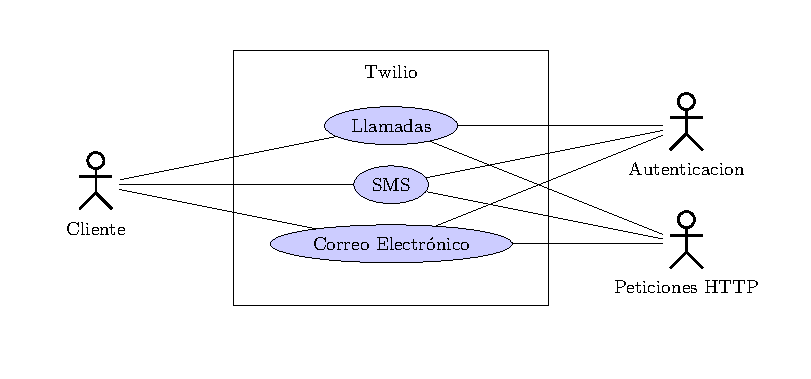
\includegraphics{usecase.pdf}

\subsection{Vista de Despliegue}

\hfill

\begin{center}
\begin{tikzpicture}[node distance=2cm]
  \node [parallelepiped,draw=black,fill=white,minimum width=5.5cm,minimum height=5cm] (Ordenador) at (0,0) {};
  \node[align=center] at (1,1.9) {<<dispositivo>>\\ \textbf{Ordenador}};

  \node[parallelepiped,draw=black,fill=white,minimum width=4.6cm,minimum height=3cm] at (-0.3,-0.6) {};
  \node[align=center] at (0.8,0.1) {<<entorno de ejecucion>>\\ \textbf{Interprete de Python}};

  \node[align=center, draw] at (0.8,-1.2) {<<artefacto>>\\ \textbf{twilio-python}};

  \node [align=center, draw]  (API) at (7,0) {<<api>>\\ \textbf{API de Twilio}};

  \draw[->] (3.46, 0) -- (5.56, 0);
 
\end{tikzpicture}
\captionof{figure}{Vista de despliegue}
\label{fig:vista de despliegue}
\end{center}

\hfill

La figura \ref{fig:vista funcional clientbase}
muestra el entorno en el que se ha de ejecutar la librería:
dentro de un intérprete de Python (ej. CPython)
en un ordenador que pueda conectarse a través de Internet
a la API de Twilio.

\subsection{Vista de Desarrollo}

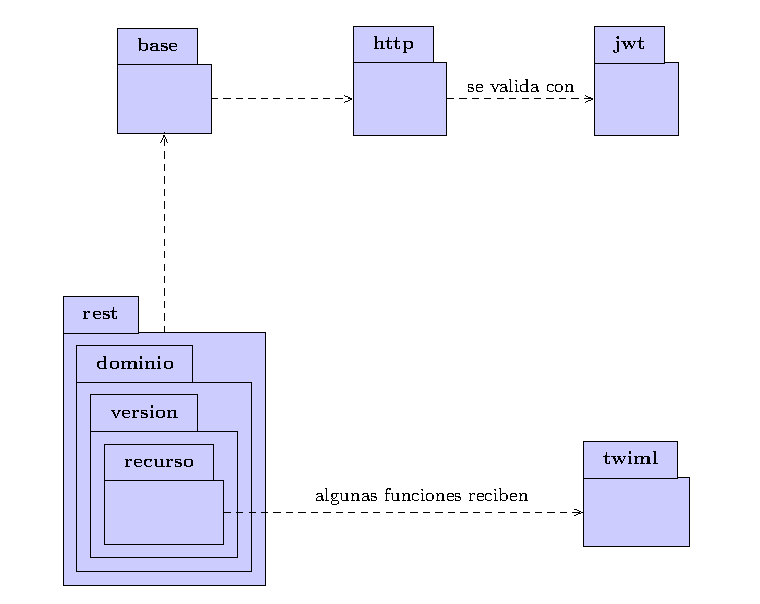
\includegraphics{vista_desarrollo.pdf}

La librería está dividida en 5 módulos.

\hfill

El módulo \verb|http| contiene diversos clientes HTTP.
Entre otros, contiene con validación usando JSON Web Tokens (JWT).
Estos permiten enviar JSONs con firma y opcionalmente encripción,
y su lógica está definida en el módulo \verb|jwt|.

\hfill

El módulo \verb|base| contiene
la lógica que usa \verb|Client|,
la clase central de la librería,
en la clase \verb|ClientBase|.
Su constructor permite configurarla,
y contiene la lógica para 
crear las cabeceras de las peticiones HTTP
con la información necesaria para autenticarlas.

También contiene las clases abstractas
para representar dominios,
las versiónes de la API que se pueden usar para un dominio
y los recursos que los dominios contienen.

\hfill

El módulo \verb|rest|
contiene toda la información específica a la API:
define todos los dominios,
todas sus versiones y todos sus recursos,
junto con sus métodos.
También extiende a \verb|ClientBase| con \verb|Client|,
añadiendo todos los dominios como parámetros
para que puedan ser accedidos.

\hfill

El módulo \verb|twiml| no depende de ningún otro.
Manualmente, se definen algunas funciones de utilidad
y la clase abstracta \verb|TwiML|
que representa una etiqueta XML.
Esta clase es extendida
con clases que representan los tipos de etiquetas especiales de TwiML.
Estas son generadas por la herramienta interna Yoyodyne
\cite{twilio-generated-yoyodyne},
en todos los lenguajes para los que Twilio mantiene librerías oficiales.
Algunos métodos de algunos recursos de \verb|rest|
reciben parámetros de tipo \verb|TwiML|.


\subsection{Vista Funcional}

\hfill

\begin{center}
  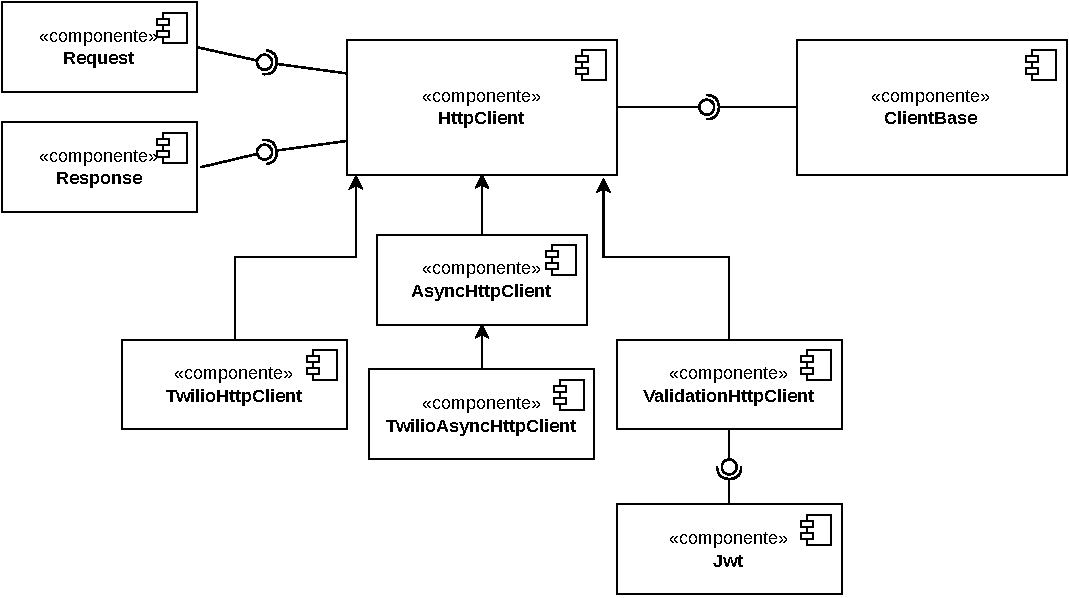
\includegraphics[width=\textwidth]{VistaFuncionalClienteBase.pdf}
  \captionof{figure}{Vista funcional de ClientBase}
  \label{fig:vista funcional clientbase}
\end{center}

\hfill


\hfill

\begin{center}
  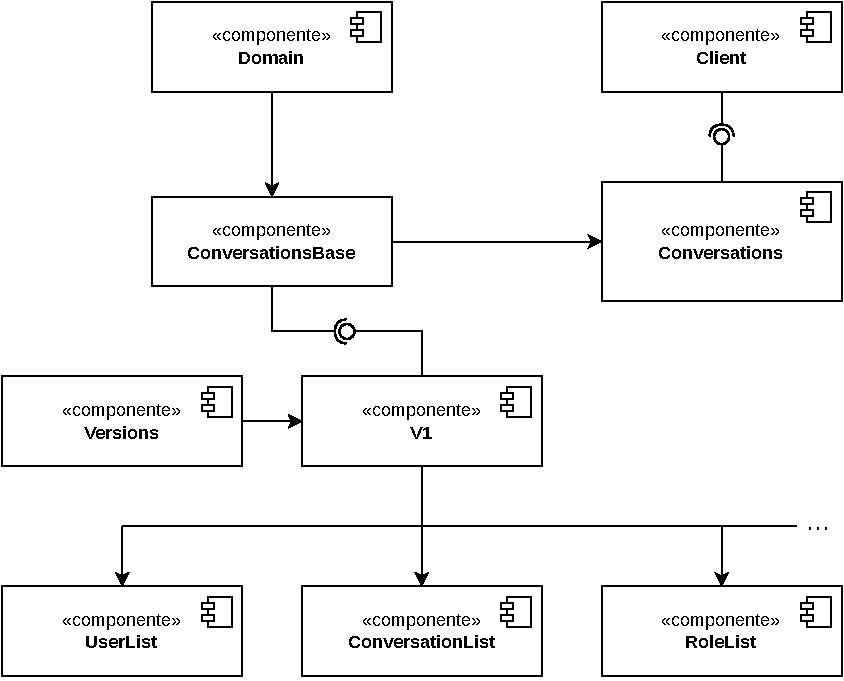
\includegraphics[width=0.9\textwidth]{VistaFuncionalDominio.pdf}
  \captionof{figure}{Vista funcional (Dominio)}
  \label{fig:vista funcional dominio}
\end{center}

\hfill

La figura \ref{fig:vista funcional dominio}
muestra la esctructura de todos los dominios
usando al dominio \verb|Conversations| como ejemplo.
La clase \verb|Conversations| implementa funciones obsoletas por retrocompatibilidad
que redirigen a las funciones de la versión con una advertencia.
La clase \verb|ConversationsBase| únicamente almacena la URL del dominio
(\verb|conversations.twilio.com|)
y una referencia a cada versión de la API
(en este caso, solo \verb|V1|).

La clase abstracta \verb|Version|
ofrece un envoltorio para el método \verb|request| de su \verb|Client|,
que toma como parámetro una URI relativa a la versión
(\verb|conversations.twilio.com/v1|)
y la realiza.
Contiene una propiedad por cada recurso que contiene el dominio.
Los diversos recursos llaman a la función \verb|request| de la versión
pasando como parámetro su URI relativa a ella, que almacenan (ej. \verb|/User|).
Para \verb|UserList|,
llamarla resulta en una petición a \verb|conversations.twilio.com/v1/User|.
Usando esto, permiten crear una instancia del recurso,
obtener una instancia del recurso,
u obtener todas las instancias
en formato de lista, de lista paginada o de \verb|stream|.



\section{Puntos de variabilidad y extensión}

La librería ofrece múltiples puntos de extensión
a través de diferentes clases abstractas.

El paquete \verb|twiml| contiene la clase abstracta \verb|TwiML|
que representa un tipo de etiqueta.

El paquete \verb|jwt| contiene la clase abstracta \verb|AccessTokenGrant|
que representa token de admisión para un recurso.

El paquete \verb|http| ofrece la clase abstracta
\verb|HttpClient|, que representa un cliente HTTP,
y su heredero abstracto \verb|AsyncHttpClient|,
que es capaz de realizar peticiones asíncronas.

En el paquete \verb|base| se definen numerosas clases abstractas:
\verb|Domain| representa un dominio
(ej. \verb|api.twilio.com|, \verb|lookups.twilio.com|),
\verb|Version| representa una versión de la API para ese dominio,
\verb|InstanceContext| representa la URI para una instancia de un recurso,
\verb|InstanceResource| representa una instancia de un recurso,
y \verb|ListResource| representa una lista de instancias de un recurso.

El paquete \verb|rest| define herederos concretos a las clases abstractas
del paquete \verb|base|, pero no contiene ningún punto de extensión.

\hfill

Esta librería ofrece puntos de variabilidad
en los argumentos que se pueden pasar
al momento de instanciar el cliente para configurarlo
\cite{readme}.
La autenticación se puede realizar con un token de autorización o
con una clave de API junto a una clave secreta.
También se puede especificar a qué región (ej. \verb|au1|)
y qué ubicación de borde (ej. \verb|sydney|)
ha de realizar peticiones el cliente.

Finalmente, se puede especificar el tipo de cliente HTTP que usa.
La librería ofrece tres clientes:
\verb|TwilioHttpClient|, el cliente síncrono por defecto,
\verb|AsyncTwilioHttpClient|, un cliente asíncrono, y
\verb|ValidationClient|, un cliente síncrono que usa encripción jwt.
Si un usuario de la librería necesitase crear un nuevo cliente,
el proceso está documentado
\cite{crear-cliente-http}.

\section{Analisis de atributos de calidad}

\subsection{Mantenibilidad}

\subsection{Fiabilidad}

\subsection{Securidad}

A pesar de que SonarCloud detecta dos problemas
(por los cuales le asigna una D).
Ambos problemas son falsos positivos, 
por lo que consideramos que la librería no tiene ningún problema de seguridad.

\hfill

SonarCloud ve que la función \verb|jwt_lib.get_unverified_header|
da acceso al contenido del JSON codificado sin verificarlo
y lo identifica como una vulnerabilidad.

\begin{lstlisting}[language=Python]
headers = jwt_lib.get_unverified_header(jwt)

alg = headers.get(alg)
if alg != cls.ALGORITHM: # cls.ALGORITHM = "HS256"
  raise ValueError(
    ...
  )

payload = jwt_lib.decode(
  ...
)
\end{lstlisting}

Sin embargo, se puede ver que no se accede al contenido.
Únicamente se verifica que el algoritmo definido en la cabecera
sea el correcto (HS256) antes de decodificar.
Se accede al contenido de manera segura.

\hfill

SonarCloud también reconoce la llamada al algoritmo SHA1,
que es inseguro \cite{sha1-broken},
como una posible vulnerabilidad.

\begin{lstlisting}[language=Python]
mac = hmac.new(self.token, s.encode("utf-8"), sha1)
\end{lstlisting}

Sin embargo, no usa el algoritmo SHA1
sino el HMAC-SHA1, que sigue siendo seguro \cite{hmac-sha1}.

\subsection{Usabilidad}

\section{Sugerencias de mejora}
En general el funcionamiento de la API es impecable debido a la generación del código, sin embargo pensamos que la documentación que aportan es bastante escueta y aporta pocos ejemplos prácticos para ayudar a nuevos usuarios a aprender a usar esta herramienta. Esto se debe a que gran parte de la documentación también es generada automáticamente.
Como sugerencia de mejora pensamos que seria buena idea añadir una documentación mas extensa, con mas ejemplos y casos de uso distintos.

\section{Contribuciones al proyecto}

Debido a lo robusta y fiable que es la librería,
no hemos encontrado ningún error en el código que se pueda arreglar.
La parte del código generada por OpenAPI-Generator
tiene una estructura confusa,
pero únicamente puede ser ajustada por empleados de Twilio \cite{contributing}.

Hemos contribuído haciendo un pull request
traduciendo el \verb|README.md| al español
\cite{contribución-readme}
y contestando a diversos issues abiertos
\cite{contribución-repeated-code}
\cite{contribución-security-improvements}
\cite{contribución-wrong-login}.

\section{Conclusiones}

En este proyecto, hemos documentado la arquitectura de Twilio-Python, el cual es un módulo python para comunicarse con la API de Twilio y generar TwiML, desarrollado por Twilio, la cual es una empresa de comunicación estadounidense.\\
Esta herramienta cuenta con un diseño basado en la arquitectura REST, que permite una gran paralelización y el caché de recursos, lo que resulta en un sistema fácil de escalar.\\
Además, gracias al estándar OpenAPI, sólo tienen que implementar una pequeña lógica, ya que sobre esa base se autogenera todo el código, lo que hace que la mantenibilidad de este sea excepcional.\\
Sin embargo, hay algunas cuestiones mejorables como la documentación, la cual es bastante escasa, ya que sólo proveen documentación de cómo crear un cliente en cada lenguaje y casos de usos básicos. \\
La forma en la que nosotros hemos contribuido con Twilio-Python ha sido traduciendo al español la documentación de cómo usar la API y respondiendo algunos de los issues abiertos.

\newpage

\printbibliography

\end{document}